\begin{frame}{Introduction}\framesubtitle{Contexte}
  \visible<+->{
    Accès à l'information numérique en domaines de spécialité.
  }

  \begin{block}<+->{Information numérique}
    \begin{itemize}
      \item{Savoir~/~Connaissance}
      \begin{itemize}
        \item{Intellectuel}
        \item{Social}
      \end{itemize}
      \item{Stockée virtuellement}
      \begin{itemize}
        \item{document électronique}
        \item{base de données électronique}
      \end{itemize}
    \end{itemize}
  \end{block}

  \begin{block}<+->{Domaine de spécialité}
    \begin{itemize}
      \item{Champ de connaissance particulier}
      \item{Possède un vocabulaire spécifique}
    \end{itemize}
  \end{block}
\end{frame}

\begin{frame}{Introduction}\framesubtitle{Contexte}
  \visible<+->{
    Valorisation de l'information numérique à l'Inist.
  }

  \begin{block}<+->{Inist (Institut de l'information scientifique et technique)}
    \begin{itemize}
      \item{Savoir faire documentaire}
      \item{Bases de données bibliographiques~:}
      \begin{itemize}
        \item{\textsc{Francis}~: Sciences humaines et sociales}
        \item{\textsc{Pascal}~: Sciences exactes}
      \end{itemize}
    \end{itemize}
  \end{block}

  \begin{block}<+->{Base de données bibliographiques}
    Collection de notices bibliographiques~:
    \begin{itemize}
      \item{Titre}
      \item{Auteur(s)}
      \item{Résumé}
      \item{Descripteurs~/~Termes-clés (mots-clés)}
    \end{itemize}
  \end{block}
\end{frame}

\begin{frame}{Introduction}\framesubtitle{Contexte}
  \begin{block}{Termes-clés}
    \begin{itemize}
      \item<1->{Unités textuelles (mots et expressions)}
      \item<1->{Décrivent le contenu d'un document}
      \item<2->{Utiles pour la Recherche d'information (\textsc{Ri})~:}
      \begin{itemize}
        \item{Indexation}
        \item{Expansion de requête}
        \item{Résumé automatique}
      \end{itemize}
      \item<3->{Utiles pour d'autres tâches~:}
      \begin{itemize}
        \item{Lecture rapide}
        \item{Aide aux dyslexiques}
      \end{itemize}
    \end{itemize}
  \end{block}
\end{frame}

\begin{frame}{Introduction}\framesubtitle{Contexte (exemple)}
  % analyse: 1
  % fouille: 1
  % oppidum: 1
  % Mailhac: 1
  % Hérault: 1
  % Aude: 1
  % Mourrel-Ferrat: 1
  % Olonzac: 1
  % répartition: 1
  % commerce: 1
  % Le Cayla: 1
  % échange: 1
  % Âge du fer: 1
  % micassé: 1
  % typologie: 2
  % chronologie: 2
  % décor: 2
  % production: 2
  % céramique: 3
  % céramique non-tournée: 3
  % distribution: 5
  % celtes: 5
  % habitat: 5
  % site fortifié: 5
  % identification: 5
  % étude du matériel: 5
  % France: 5
  % Europe: 5
  % La Tène: 5
  \begin{exampleblock}{\small
    Étude préliminaire de la \textbf{\normalsize céramique non tournée}
    \textbf{\normalsize micacée} du bas Languedoc occidental~:
    \textbf{\normalsize typologie}, \textbf{\normalsize chronologie} et aire de
    diffusion
  }\justifying\small
    \alt<2>{
      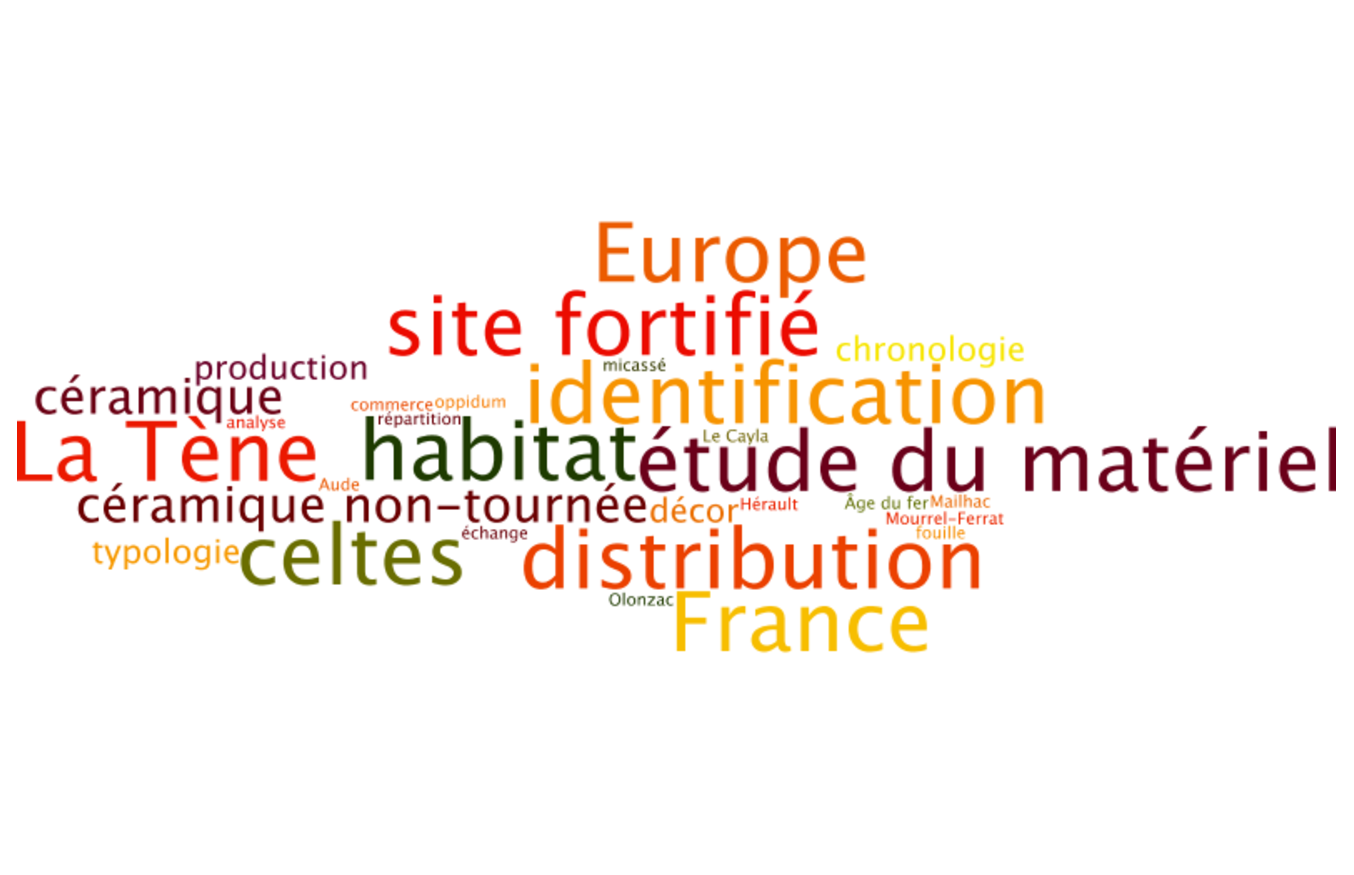
\includegraphics[width=\linewidth]{include/exemple_archeologie.eps}
    }{
      L'étude présente une variété de \textbf{\normalsize céramique non tournée}
      dont la \textbf{\normalsize typologie} et l'\textbf{\normalsize analyse} des
      \textbf{\normalsize décors} permettent de l'identifier facilement. La nature
      de l'argile enrichie de mica donne un aspect pailleté à la pâte sur laquelle
      le \textbf{\normalsize décor} effectué selon la méthode du brunissoir
      apparaît en traits brillant sur fond mat. Cette première approche se fonde
      sur deux séries issues de \textbf{\normalsize fouilles} anciennes menées sur
      les \textbf{\normalsize oppidums} du \textbf{\normalsize Cayla} à
      \textbf{\normalsize Mailhac} (\textbf{\normalsize Aude}) et de
      \textbf{\normalsize Mourrel-Ferrat} à \textbf{\normalsize Olonzac}
      (\textbf{\normalsize Hérault}). La carte de \textbf{\normalsize répartition}
      fait état d'\textbf{normalsize échanges} ou de \textbf{\normalsize commerce}
      à l'échelon macrorégional rarement mis en évidence pour de la
      \textbf{\normalsize céramique non tournée}. S'il est difficile de statuer
      sur l'origine des \textbf{\normalsize décors}, il semble que la
      \textbf{\normalsize production} s'insère dans une ambiance celtisante. La
      \textbf{\normalsize chronologie} de cette \textbf{\normalsize production} se
      situe dans le deuxième \textbf{\normalsize âge du Fer}. La fourchette
      proposée entre la fin du IV$^\text{e}$ et la fin du II$^\text{e}$ s. av.
      J.-C. reste encore à préciser.
    }
  \end{exampleblock}
\end{frame}

